\documentclass{article}

\usepackage[margin=1in]{geometry}
\usepackage{fancyhdr}
\usepackage{amsmath}
\usepackage{amssymb}
\usepackage{listings}
\usepackage{graphicx}
\usepackage{enumerate}
\usepackage{tikz}
\usetikzlibrary{automata,positioning}


\pagestyle{fancy}

\lhead{CS 373 \\ Homework 3}
\chead{}
\rhead{Drew Cross (ddcross2) \\ \emph{partners}: Eric Parsons}
\lfoot{}
\cfoot{}
\rfoot{}

\begin{document}

\subsection*{Problem 1}
Prove that the following languages are non-regular using the Myhill-Nerode theorem.
\begin{enumerate}[(a)]

\item $A = \{ww\ |\ w \in \Sigma^*\}$ over the alphabet $\Sigma = \{0,1\}$. (5 Points)

\textbf{Claim:}
    $A = \{ww\ |\ w \in \Sigma^*\}$ over the alphabet $\Sigma = \{0,1\}$ is nonregular.\\
\textbf{Proof:}
    Consider the equivalence relation $\sim_A$ on $A$ and the set of strings \\
    $S = \{10^n | n \geq 0 \}$ \\
    For $x = 10^i$ and $y = 10^j$ where $i \neq j$, \\
    Notice that $\exists z = 10^i$ S.T. $xz \in A$ but
    $yz \notin A$ \\
    Thus $x$ and $y$ belong to separate equivalence classes,
    and each equivalence class for a string in
    $A$ is distinct from the others. Since $S$ is infinite, there must be an infinite number of
    equivalence classes, implying that $A$ is nonregular by the Myhill-Nerode theorem.
    \[ \square \]

\item $B = \{w \in \Sigma^*\ |\ \#0(w) = 2 $ or $ \#2(w) < \#0(w)\}$ over the alphabet
    $\Sigma = \{0,1,2\}$. (5 Points)

\textbf{Claim:}
    $B = \{w \in \Sigma^*\ |\ \#0(w) = 2 $ or $ \#2(w) < \#0(w)\}$ over the alphabet
    $\Sigma = \{0,1,2\}$ is nonregular.\\
\textbf{Proof:}
    Consider the equivalence relation $\sim_B$ on $B$ and the set of strings \\
    $S = \{0^n | n \geq 0 \}$ \\
    For $x = 00^i$ and $y = 00^j$ and $i \neq j$ Without the loss of generality assume
    $i > j$.*\\
    Notice that $\exists z=2^i$ S.T. $xz \in B$ but $yz \notin B$. \\
    Thus $x$ and $y$ belong to separate equivalence classes,
    and each equivalence class for a string in
    $B$ is distinct from the others. Since $S$ is infinite, there must be an infinite number of
    equivalence classes, implying that $B$ is nonregular by the Myhill-Nerode theorem.

    *(If $i < j$ then $xz \notin B$ and $yz \in B$)\\
    \[ \square \]

\item $C = \{x=y+z | x,y,z$ are natural numbers base 10, and $x$ is the sum of $y$ and $z\}$
    over the alphabet $\Sigma = \{0,1,2,3,4,5,6,7,8,9,+,=\}$. For example, the string
    "15=4+11" is in $C$, but "5=2+2" and "3=3" are not. (5 Points)

\textbf{Claim:}
    $C = \{x=y+z\ |\ x,y,z$ are natural numbers base 10, and $x$ is the sum of $y$ and $z\}$
    is nonregular.
\textbf{Proof:}
    Consider the equivalence relation $\sim_C$ on $C$ and the set of strings \\
    $S = \{ 10^{2n}1 = 1+10^n | n \geq 1\}$
    %TODO
    For $x = 10^{2i}1 = 1 + 10^i \in S$ and $y = 10^{2j} + 10^j \in S$ \\
    Notice there is a string $z = 0^{i+1}$ such that $xz \in S$ but $yz \notin S$ \\
    Thus $x$ and $y$ belong to separate equivalence classes,
    and each equivalence class for a string in
    $B$ is distinct from the others. Since $S$ is infinite, there must be an infinite number of
    equivalence classes, implying that $B$ is nonregular by the Myhill-Nerode theorem.
    \[ \square \]


\end{enumerate}

\newpage


\subsection*{Problem 2}
In a context-free grammar $G = (V, \Sigma, R, S)$, a variable $A \in V$ is called cyclic if for some $u,v \in
(V \cup \Sigma)^*$ there exists a sequence of derivations $A \Rightarrow w_1 \Rightarrow w_2 \Rightarrow$ ... 
$ \Rightarrow w_k \Rightarrow uAv,k \geq 0$. Grammar $G$ is cyclic if at least one of its variables is cyclic,
otherwise $G$ is cycle-free.
\begin{enumerate}[(a)]
\item Prove that the language generated by a cycle-free grammar is finite. (10 Points)

%TODO
A Language generated by a cycle-free grammar is finite because a grammar contains a finite
number of rules. Because there are no cycles, we can take one of the derivations for the start state
and replace each variable on the right side with its production. We can now "push down" the chosen
variable into each of the other rules. Since there are no cycles, we can do this for each variable
until we are left with terminals only. If there were cycles we would find a point where "pushing
down" the variables would become futile, because we would just keep expanding the strings. Now
that we have removed all variables, we have our start variable going to a set of strings, which
exactly describes our language. For example: \\

\begin{minipage}[c]{0.5\linewidth}
$S \rightarrow A\ |\ B$ \\
$A \rightarrow C\ |\ D$ \\
$B \rightarrow E\ |\ A$ \\
$C \rightarrow aa\ |\ bb$ \\
$D \rightarrow a\ |\ b$ \\
$E \rightarrow aba\ |\ bab$ \\
\textbf{Replacing A:}\\
$S \rightarrow C\ |\ D\ |\ B$ \\
$B \rightarrow E\ |\ C\ |\ D$ \\
$C \rightarrow aa\ |\ bb$ \\
$D \rightarrow a\ |\ b$ \\
$E \rightarrow aba\ |\ bab$ \\
\textbf{Replacing C:} \\
$S \rightarrow aa\ |\ bb\ |\ D\ |\ B$ \\
$B \rightarrow E\ |\ aa\ |\ bb\ |\ D$ \\
$D \rightarrow a\ |\ b$ \\
$E \rightarrow aba\ |\ bab$ \\
\end{minipage}
\begin{minipage}[c]{0.5\linewidth}
\textbf{Replacing D:} \\
$S \rightarrow aa\ |\ bb\ |\ a\ |\ b\ |\ B$ \\
$B \rightarrow E\ |\ aa\ |\ bb\ |\ a\ |\ b$ \\
$E \rightarrow aba\ |\ bab$ \\
\textbf{Replacing B:}\\
$S \rightarrow aa\ |\ bb\ |\ a\ |\ b\ |\ E\ |\ aa\ |\ bb\ |\ a\ |\ b$ \\
$E \rightarrow aba\ |\ bab$ \\
\textbf{Replacing E:}\\
$S \rightarrow aa\ |\ bb\ |\ a\ |\ b\ |\ aba\ |\ bab\ |\ aa\ |\ bb\ |\ a\ |\ b$ \\
\end{minipage}

\item Is it necessarily true that the language generated by a cyclic grammar is infinite? Explain your
answer. (5 Points).

%TODO
No, If a language cycles with only variables. For example the grammar $A$: \\
$A \rightarrow B $ \\
$B \rightarrow C $ \\
$C \rightarrow A\ |\ ab$



\end{enumerate}

\newpage


\subsection*{Problem 3}
Construct CFGs for the following languages. Give a brief explanation of how your
grammar works and what each nonterminal stands for. The CFGs must be designed
by hand and not converted from PDAs using the equivalence theorem.

\begin{enumerate}[(a)]
\item $A = \{0^m1^n\ |\ m > n \geq 0$ and $ m - n$ is even$\}$. (5 Points)

$S \rightarrow A$ \\
$A \rightarrow 00\ |\ 0A1\ |\ 00A $\\


\item The compliment of $B = \{0^n1^n | n \geq 0\}$ over the alphabet $\Sigma = \{0,1\}$. (5 Points)

$S \rightarrow\ A\ |\ B\ |\ C10C $ \\
$A \rightarrow\ 0\ |\ 0A\ |\ 0A1 $ \\
$B \rightarrow\ 1\ |\ B1\ |\ 0B1 $ \\
$C \rightarrow\ 0C\ |\ 1C |\ \varepsilon $


\item $C = \{0^m1^n2^k3^l | m+n=k+l, m,n,k,l \geq 0\}$. (5 Points)

%TODO
$S \rightarrow 0S3\ |\ B\ |\ C $ \\
$B \rightarrow 0B2\ |\ D $ \\
$C \rightarrow 1C2\ | D $ \\
$D \rightarrow 1D2\ |\ \varepsilon$

\end{enumerate}

\newpage


\subsection*{Problem 4}
Construct PDAs for the following languages and explain how htey work. The PDAs must be designed by hand and
not converted from CFGs using the equivalence theorem.

\begin{enumerate}[(a)]
\item $A = \{ 0^n1^{2n+m}0^{m-1} | m,n \in \mathbb{N}\}$. (5 Points)
%TODO
\item $B = \{ w \in \{0,1\}^* | \#0(w) > \#1(w)$ and $(\#0(w) - \#1(w))$ is even $\}$. (5 Points)
%TODO
\item The compliment of $C = \{ww | w\in \Sigma^*\}$ over the alphabet $\Sigma = \{0,1\}$. (10 Points)

        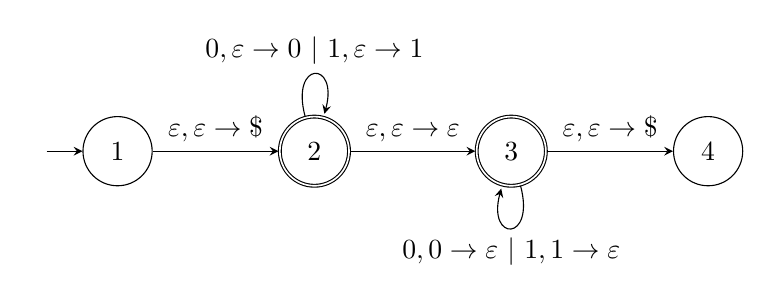
\begin{tikzpicture}[%
        >=stealth,
        node distance=2.5cm,
        on grid,
        auto
        ]

        \node[initial,initial text=,state] (1)  {1};
        \node[state, accepting] (2) [right of=1] {2};
        \node[state, accepting] (3) [right of=2] {3};
        \node[state] (4) [right of=3] {4};

        \path[->] (1) edge node {$\varepsilon, \varepsilon \rightarrow \$$} (2);
        \path[->] (2) edge[loop above] node {$0, \varepsilon \rightarrow 0\ | $
                                             $1, \varepsilon \rightarrow 1$
                                             } (2);
        \path[->] (2) edge node {$\varepsilon, \varepsilon \rightarrow \varepsilon $} (3);
        \path[->] (3) edge[loop below] node {$0, 0 \rightarrow \varepsilon\ | $
                                             $1, 1 \rightarrow \varepsilon$
                                             } (3);
        \path[->] (3) edge node {$\varepsilon, \varepsilon \rightarrow \$$} (4);

        \end{tikzpicture}
%TODO
\end{enumerate}

\newpage


\subsection*{Problem 5}
        Recall that in our definition of a PDA, the transition function was described as $\delta: Q\times\Sigma_\varepsilon\times\Gamma_\varepsilon\to\mathcal{P}(Q\times\Gamma_\varepsilon)$. In an attempt to advance the human knowledge in the field of theoretical computer science, Professor Professorson\footnote{All characters appearing in this problem are fictional. Any resemblance to other persons, real or fictional, is purely coincidental.} has introduced a new concept, an extended pushdown automaton (EPDA).
        
        An EPDA is defined in the same way as a PDA, except for the transition function component, which is now given as $\delta: Q\times\Sigma_\varepsilon\times\Gamma_\varepsilon\to\mathcal{P}(Q\times\Gamma^*)$. In other words, an EPDA can push a string of multiple characters onto the stack in a single transition. 
        
        Professor Professorson believes that EPDAs are equivalent to PDAs (and thus to CFGs), but are easier to construct. If true, his idea can revolutionize the industry of PDA generation.
        \begin{enumerate}[(a)]
    \item Prove the professor wrong. In fact, show that for \textit{any} language $L\subseteq\Sigma^*$,
            some EPDA recognizes it. (10 Points)
    \item Shocked by our previous result, the professor claims that he can prove the equivalence of EPDAs and PDAs.
    Actually, we have already used the shorthand notation for pushing an entire string onto the stack in the proof of
    the PDA--CFG equivalence theorem. 

            For example, any transition of the form $\delta(q,a,s)\ni(r,xyz)$ can be rewritten as a series of one-character transitions by adding extra states: $\delta(q,a,s)\ni(q_1,x)$, $\delta(q_1,\varepsilon,\varepsilon)=\{(q_2,y)\}$, $\delta(q_2,\varepsilon,\varepsilon)=\{(r,z)\}$ (for more details and a picture, see the lecture notes or Sipser, pages 116--117).
            
            According to Professor Professorson, this allows us to convert any EPDA into an equivalent PDA. Explain how this construction does not contradict the existence of non-context free languages. (5 Points)
%TODO
\end{enumerate}

\newpage


\subsection*{Problem 6}
Consider grammar $G = (\{$S,A,B$\},\{0,1\}$,R,S), where
\[
    S \rightarrow AB\ |\ BA
\]
\[
    A \rightarrow 0\ |\ 0A0\ |\ 0A1\ |\ 1A0\ |\ 1A1 \\
\]
\[
    B \rightarrow 1\ |\ 0B0\ |\ 0B1\ |\ 1B0\ |\ 1B1 \\
\]

\begin{enumerate}[(a)]
\item What language does this grammar generate? Give a simple description with little
or no mathematical notation (no more than 15-20 words). (7 Points) \\
The set of all pairs of strings that are odd length, whose central symbols are not the same, concatenated together.

\item Prove your answer to part (a). That is, prove that every string of the language
can be derived in G, and that every string that can be derived is in the language. (10 Points)
%TODO

\item Is G ambiguous? If your answer is yes", give an example of a string with 2
different derivations. (3 Points)

Yes: \\
$S \Rightarrow AB \Rightarrow 0A0B \Rightarrow 000B \Rightarrow
0001B1 \Rightarrow 000111$ \\
and \\
$S \Rightarrow AB \Rightarrow 0A1B \Rightarrow 00A11B \Rightarrow
00011B \Rightarrow 000111$
\end{enumerate}

\end{document}
